\documentclass[tikz,border=2pt]{standalone}
% Shared Figure architecture visual system for all four main-text figures.
\usepackage[T1]{fontenc}
\usepackage{charter}
\usepackage[scaled=0.90]{helvet}
\usepackage{amsmath,amssymb}
\renewcommand{\Pr}{\mathbb{P}}
\usepackage{xcolor}
\usepackage{tikz}
\usepackage{pgfplots}
\pgfplotsset{compat=1.18}
\usetikzlibrary{arrows.meta,calc,positioning,fit,decorations.pathreplacing,shapes.geometric,backgrounds}
\definecolor{figNavy}{RGB}{0,63,92}
\definecolor{figBlue}{RGB}{0,101,165}
\definecolor{figSky}{RGB}{226,241,249}
\definecolor{figTeal}{RGB}{0,125,112}
\definecolor{figMint}{RGB}{224,243,239}
\definecolor{figOrange}{RGB}{222,102,35}
\definecolor{figPeach}{RGB}{252,235,224}
\definecolor{figRed}{RGB}{145,43,55}
\definecolor{figInk}{RGB}{35,45,51}
\definecolor{figGray}{RGB}{103,115,123}
\definecolor{figRule}{RGB}{194,202,208}
\definecolor{figPale}{RGB}{248,250,251}
\definecolor{figWhite}{RGB}{255,255,255}
\tikzset{
  figpanel/.style={draw=figRule,line width=0.55pt,rounded corners=2.4pt,fill=figWhite},
  figtag/.style={circle,fill=figBlue,text=figWhite,minimum size=4.3mm,inner sep=0pt,font=\sffamily\bfseries\fontsize{7.5}{8}\selectfont},
  figtitle/.style={font=\sffamily\bfseries\fontsize{8.5}{10}\selectfont,text=figNavy,anchor=west},
  figsubtitle/.style={font=\sffamily\fontsize{6.8}{8}\selectfont,text=figGray,align=left},
  figbody/.style={font=\sffamily\fontsize{7}{8.4}\selectfont,text=figInk,align=center},
  figsmall/.style={font=\sffamily\fontsize{6.2}{7.4}\selectfont,text=figGray,align=center},
  figmath/.style={font=\fontsize{7.4}{8.8}\selectfont,text=figInk,align=center},
  figflow/.style={-{Stealth[length=2.0mm,width=1.4mm]},draw=figBlue,line width=0.85pt},
  figflowgray/.style={-{Stealth[length=1.8mm,width=1.25mm]},draw=figGray,line width=0.75pt},
  figfloworange/.style={-{Stealth[length=2.0mm,width=1.4mm]},draw=figOrange,line width=0.85pt},
  figbluebox/.style={draw=figBlue,line width=0.65pt,fill=figSky,rounded corners=2.2pt},
  figorangebox/.style={draw=figOrange,line width=0.65pt,fill=figPeach,rounded corners=2.2pt},
  figtealbox/.style={draw=figTeal,line width=0.65pt,fill=figMint,rounded corners=2.2pt},
  figgraybox/.style={draw=figRule,line width=0.6pt,fill=figPale,rounded corners=2.2pt},
}
\newcommand{\PanelHeading}[4]{%
  \node[figtag] at (#1,#2) {#3};%
  \node[figtitle] at ({#1+0.32},#2) {#4};%
}

\begin{document}
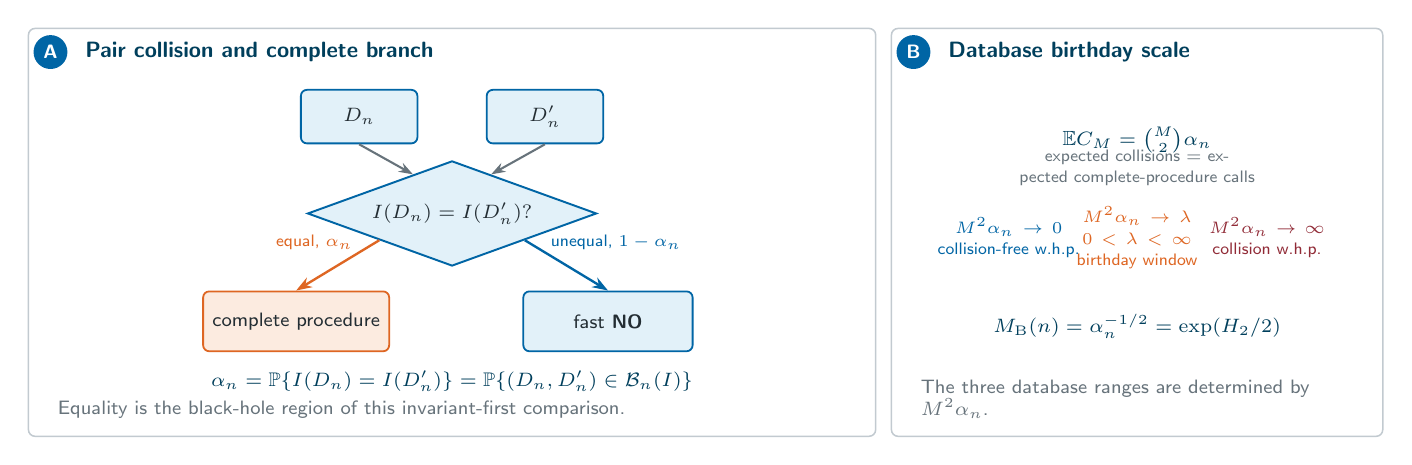
\begin{tikzpicture}[x=1cm,y=1cm]
% Overall dimensions: 17.2 cm x 5.18 cm.
\draw[figpanel] (0,0) rectangle (10.76,5.18);
\draw[figpanel] (10.96,0) rectangle (17.20,5.18);

% Panel A: one equality event, read from top to bottom.
\PanelHeading{0.28}{4.88}{A}{Pair collision and complete branch}

\node[figbluebox,minimum width=1.48cm,minimum height=0.68cm,figbody] (aD) at (4.20,4.06) {$D_n$};
\node[figbluebox,minimum width=1.48cm,minimum height=0.68cm,figbody] (aDp) at (6.56,4.06) {$D_n'$};
\node[diamond,draw=figBlue,fill=figSky,line width=0.7pt,aspect=2.75,
      minimum width=3.18cm,minimum height=0.76cm,figbody] (atest) at (5.38,2.83)
      {$I(D_n)=I(D_n')?$};
\node[figorangebox,minimum width=2.15cm,minimum height=0.76cm,figbody] (afallback) at (3.40,1.46)
      {complete procedure};
\node[figbluebox,minimum width=2.15cm,minimum height=0.76cm,figbody] (ano) at (7.36,1.46)
      {fast \textbf{NO}};

\draw[figflowgray] (aD.south) -- (atest.135);
\draw[figflowgray] (aDp.south) -- (atest.45);
\draw[figfloworange] (atest.south west) -- (afallback.north);
\draw[figflow] (atest.south east) -- (ano.north);
\node[font=\sffamily\fontsize{6.2}{7.4}\selectfont,text=figOrange,anchor=south east]
  at (4.24,2.24) {equal, $\alpha_n$};
\node[font=\sffamily\fontsize{6.2}{7.4}\selectfont,text=figBlue,anchor=south west]
  at (6.51,2.24) {unequal, $1-\alpha_n$};

\node[font=\fontsize{7.1}{8.4}\selectfont,text=figNavy] at (5.38,0.70)
  {$\alpha_n=\mathbb P\{I(D_n)=I(D_n')\}
   =\mathbb P\{(D_n,D_n')\in\mathcal B_n(I)\}$};
\node[figsubtitle,anchor=south west,text width=10.05cm] at (0.25,0.10)
  {Equality is the black-hole region of this invariant-first comparison.};

% Panel B: database workload and inverse-birthday regimes.
\PanelHeading{11.24}{4.88}{B}{Database birthday scale}

\node[figmath,text=figNavy] at (14.08,3.76)
  {$\mathbb E C_M=\binom{M}{2}\alpha_n$};
\node[figsmall,text width=5.25cm] at (14.08,3.41)
  {expected collisions $=$ expected complete-procedure calls};
\node[font=\sffamily\fontsize{6.4}{7.7}\selectfont,text=figBlue,align=center,text width=1.82cm]
  at (12.45,2.52) {$M^2\alpha_n\to0$\\collision-free w.h.p.};
\node[font=\sffamily\fontsize{6.4}{7.7}\selectfont,text=figOrange,align=center,text width=1.82cm]
  at (14.08,2.52) {$M^2\alpha_n\to\lambda$\\$0<\lambda<\infty$\\birthday window};
\node[font=\sffamily\fontsize{6.4}{7.7}\selectfont,text=figRed,align=center,text width=1.82cm]
  at (15.73,2.52) {$M^2\alpha_n\to\infty$\\collision w.h.p.};

\node[figmath,text=figNavy] at (14.08,1.40)
  {$M_{\mathrm B}(n)=\alpha_n^{-1/2}=\exp(H_2/2)$};
\node[figsubtitle,anchor=south west,text width=5.55cm] at (11.21,0.10)
  {The three database ranges are determined by $M^2\alpha_n$.};
\end{tikzpicture}
\end{document}
